\textbf{Tableau récapitulatif des réponses}

\begin{center}

		\begin{tblr}{hlines,vlines,colspec={c*{9}{c}},cells={c,m},row{1}={font=\bfseries}}
			Question & 1 & 2 & 3 & 4 & 5 & 6 & 7 & 8 & 9 \\
			Réponse  & B & B & D & C & B & C & B & C & B \\
		\end{tblr}
	\end{center}

	\medskip

	\textbf{Justifications}

	\begin{enumerate}
		\item \textbf{Bonne réponse : B.}

		$\dfrac{1}{2}+\dfrac{3}{2}\times 4= \dfrac{1}{2}+\dfrac{12}{2}=\dfrac{13}{2}$.

		\item \textbf{Bonne réponse : B.}

		La partie visible ($\np[km^3]{150}$) représente $10~\%$ du volume total $V$.

		Donc \quad $0,10 \times V = 150 \iff V=\dfrac{150}{0,10}=\np[km^3]{1500}$.

		\item \textbf{Bonne réponse : D.}

		$0,845=1-0,155 = 1 + \dfrac{-15,5}{100}$ : le coefficient multiplicateur $0,845$ est donc associé à une évolution dont le taux est de $-15,5~\%$, c'est donc une baisse de $15,5~\%$.

		\item \textbf{Bonne réponse : C.}

		$A(x)=(x+5)(x+8)$ est un polynome du second degré, qui s'annule en $-5$ et $-8$.

		Il est présenté sous sa forme factorisée, avec un coefficient dominant positif (égal à 1), donc les valeurs prises par ce polynome sont positives, sauf entre les deux racines.

		On pouvait aussi établir le tableau de signe à partir du signe des facteurs de degré 1 :

		\begin{center}
				\begin{tikzpicture}
					\tkzTabInit[lgt=1.5,espcl=1.4]
					{$x$/0.7,$x+8$/0.7,$x+5$/0.7,$A(x)$/0.7}
					{$-\infty$,$-8$,$-5$,$+\infty$}
				\tkzTabLine{,-,z,+,,+,}
				\tkzTabLine{,-,,-,z,+,}
				\tkzTabLine{,+,z,-,z,+,}
			\end{tikzpicture}
		\end{center}

		\item Les lettres du mot SINGE sont $\{$S, I, N, G, E$\}$ : $5$ lettres, dont $2$ voyelles (I et E).

		Puisque le singe choisit une lettre au hasard, on est en situation d'équiprobabilité, chaque lettre a autant de chance qu'une autre d'être choisie.

		$P_{M}(V)=\dfrac{\text{nombre de voyelles dans SINGE}}{\text{nombre de lettres de SINGE}}=\dfrac{2}{5}$.

		\item \textbf{Bonne réponse : C.}

		La droite passe par les points $(0 ; 30)$ et $(3 ; 0)$.

		L'ordonnée à l'origine est donc : \quad $30$.

		Le coefficient directeur est donné par :\quad $\dfrac{0-30}{3-0}=-10$.

		Donc la fonction représentée a bien pour expression :\quad $f(x)=-10x+30$.

		\item \textbf{Bonne réponse : B.}

		 $\begin{aligned}
		 	(x+2)^{2}-(1-x)^{2}&=\left(x^{2}+4x+4\right)-\left(1-2x+x^{2}\right)\\
		 	&=x^{2}+4x+4-1+2x-x^{2}\\
		 	&=6x+3
		 \end{aligned}$

		\item \textbf{Bonne réponse : C.}

		$\forall x \in \R$,\quad $2(x-4)-(2x+1)=2x-8-2x-1=-9$.

		L'égalité \quad $-9=0$ \quad est fausse, et ce pour tout réel $x$, puisqu'elle ne dépend pas de $x$ : l'équation n'admet aucune solution.

		\item \textbf{Bonne réponse : B.}

		$E=\dfrac{2\times 3^{2}}{27\times 2^{3}}
		=\dfrac{2\times 3^2}{3^3\times 2^3}
		=\dfrac{2^0 \times 3^0}{2^2 \times 3^1}
		=\dfrac{1}{4\times 3}
		=\dfrac{1}{12}$.
	\end{enumerate}
